\hypertarget{group__appbx}{}\section{Application box(es)}
\label{group__appbx}\index{Application box(es)@{Application box(es)}}
One or more boxes that run applications (e.\+g. V\+I\+SA, E\+MV, Mastercard, Main application, etc) may exist and leverage R\+PC A\+PI of other boxes (Boxes can communicate with each other through Remote Procedure Calls aka R\+PC).

Their identification (box ID) will grant them access to their private data or specific privileges when using the A\+PI.

Those boxes run in independent threads.

P\+R\+I\+V\+I\+L\+E\+GE L\+E\+V\+EL\+: \char`\"{}\+Box Trusted\char`\"{} or \char`\"{}\+Box Other\char`\"{}

They actually implement the high-\/level services proposed by the device (e.\+g. payment application). By using the Secure Sandbox services box and the P\+CI Security Services box, the applications may be kept out of the certification perimeter. Code can also run out of any box.


\begin{DoxyImageNoCaption}
  \mbox{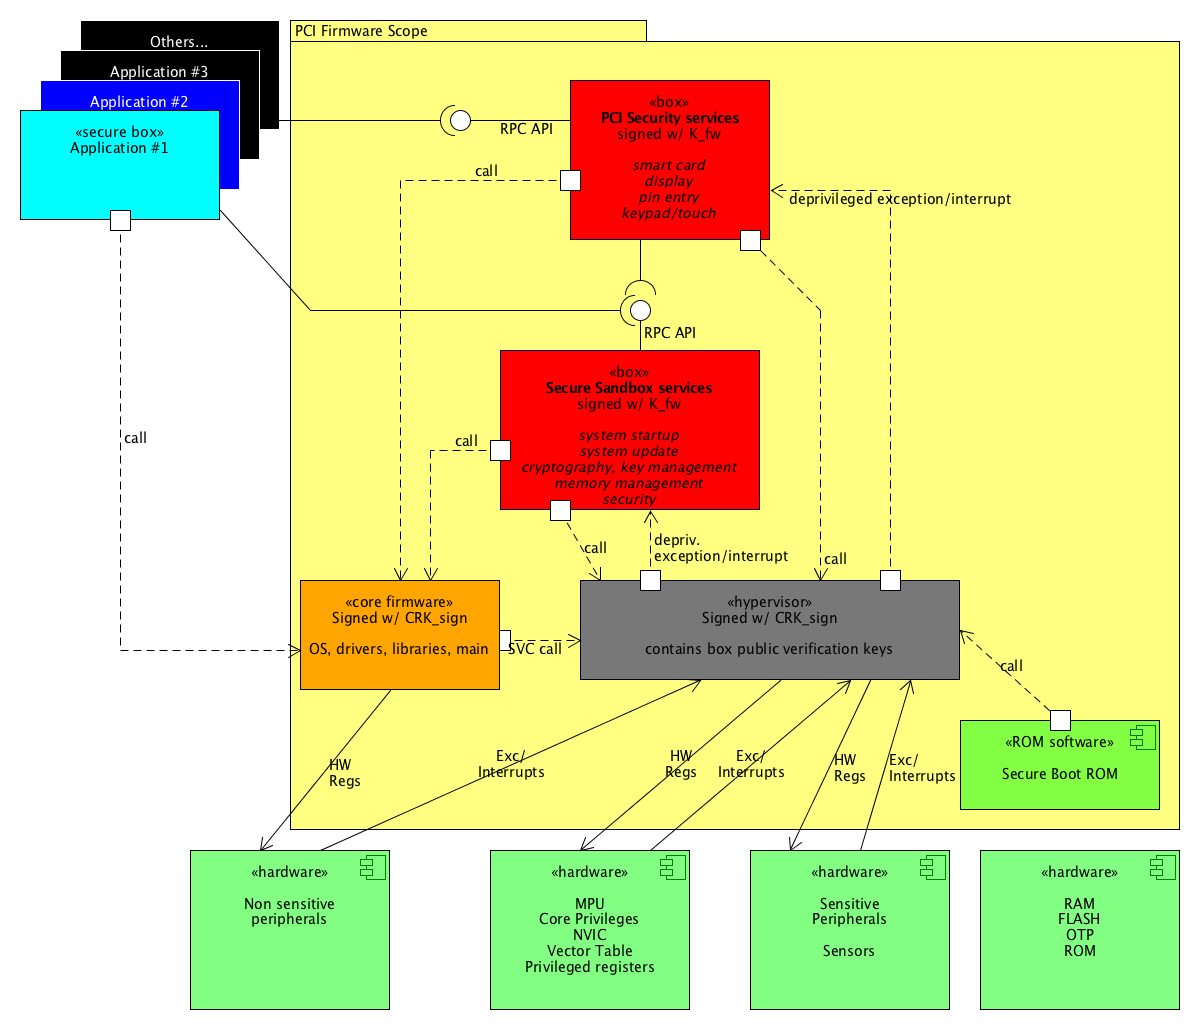
\includegraphics[width=\textwidth,height=\textheight/2,keepaspectratio=true]{pci_cortex.png}}
\end{DoxyImageNoCaption}
  